\section{Related Work}
\label{sec:related}

\subsection{Explainability and counterfactual model probing}

Many post-hoc image explanations assign importance to pixels or regions. Their reliability depends on whether the explanation actually changes with the learned model, a point made explicit by saliency-map sanity checks~\cite{adebayo2018sanity} and by work on explainability in precision pathology~\cite{klauschen2024xai}. Counterfactual explanations take a different form: they search for a nearby input with a different prediction. Goyal \etal{} use discriminative visual comparisons~\cite{goyal2019counterfactual}. DVCE and DiME place classifier-guided edits under diffusion image priors~\cite{augustin2022dvce,jeanneret2022dime}, and DiG-IN extends diffusion guidance to comparisons between networks and neuron-level visualization~\cite{augustin2024digin}.

Interventions have also been used to examine the generative model itself. Tinaz \etal{} fit sparse autoencoders to diffusion activations, identify concepts at different denoising stages, and manipulate image composition and style through those concepts~\cite{tinaz2025concepts}. This line of work is useful for understanding where a generative representation forms. Our experiments instead use a conditional generator as an input instrument for testing external pathology models.

Histopathology counterfactual methods include synthetic class transitions linked to molecular labels~\cite{dolezal2023synthetic} and MoPaDi, which couples a diffusion autoencoder~\cite{preechakul2022diffae} to classifiers and multiple-instance models to edit morphology toward a target prediction~\cite{zigutyte2026mopadi}. These approaches motivate biologically plausible edits. Our evaluation additionally requires the requested intervention to be recovered from the generated image before that image is used for model probing.

\subsection{Pathology representations and cellular analysis}

TCGA made matched pathology and molecular data available across tumor types and institutions~\cite{tcga2013pancancer}. Pathology representation learning has since progressed from transformer-based contrastive pretraining to large-scale visual and image--language foundation models~\cite{wang2022ctranspath,chen2024uni,vorontsov2024virchow,lu2024conch,xu2024gigapath}. These models support many downstream tasks, but benchmark accuracy alone does not identify whether a response comes from morphology, cell layout, stain, or another feature. We therefore treat pretrained encoders as models to audit with controlled inputs.

The controls and measurements in this paper depend on cell-level structure. HoVer-Net jointly segments and classifies nuclei in multi-tissue histology~\cite{graham2019hovernet}. StarDist detects instances using star-convex polygons~\cite{schmidt2018stardist}, while CellViT++ combines a foundation-model encoder with efficient cell segmentation and classification~\cite{horst2026cellvitpp}. These models disagree in taxonomy and boundary placement. We use that disagreement deliberately: CellViT++ participates in candidate selection, while HoVer-Net and StarDist provide out-of-loop measurements.

\subsection{Controllable histopathology generation}

PathologyGAN learned realistic tissue structure and interpretable latent representations with a generative adversarial model~\cite{quiros2021pathologygan}. PathLDM introduced text-conditioned latent diffusion for histopathology patches~\cite{yellapragada2024pathldm}; Harb \etal{} extended diffusion synthesis to gigapixel WSIs~\cite{harb2024gigapixel}; and Spatial Diffusion modeled explicit cell layouts~\cite{li2024spatialdiffusion}. Together, these studies show the increasing control available in histopathology generation; our focus is whether a requested change is recovered reliably enough for counterfactual model analysis.

Latent diffusion performs denoising in a compressed image representation~\cite{rombach2022latent}, while ControlNet and FiLM provide complementary mechanisms for spatial and feature-wise conditioning~\cite{zhang2023controlnet,perez2018film}. These mechanisms support separate interventions on cellular organization and morphology or appearance; the central evaluation question is whether the generated image faithfully reflects each requested change.

\subsection{Realism, condition fidelity, and auditing}

FID~\cite{heusel2017fid} and KID~\cite{binkowski2018kid} compare generated and reference feature distributions. Neither metric tests adherence to a spatial map or morphology vector. A generator can score well while placing the wrong cell type, missing a requested count, or changing stain together with nuclear shape.

We report realism and condition fidelity separately. Spatial checks use recovered counts and centroid agreement. Morphology is measured across images and again within the same source image over a five-level dose sweep. Downstream probing is restricted to pairs that pass the generation-side checks. Figure~\ref{fig:overview} shows where selection and independent auditing enter the pipeline.

\begin{figure*}[!t]
    \centering
    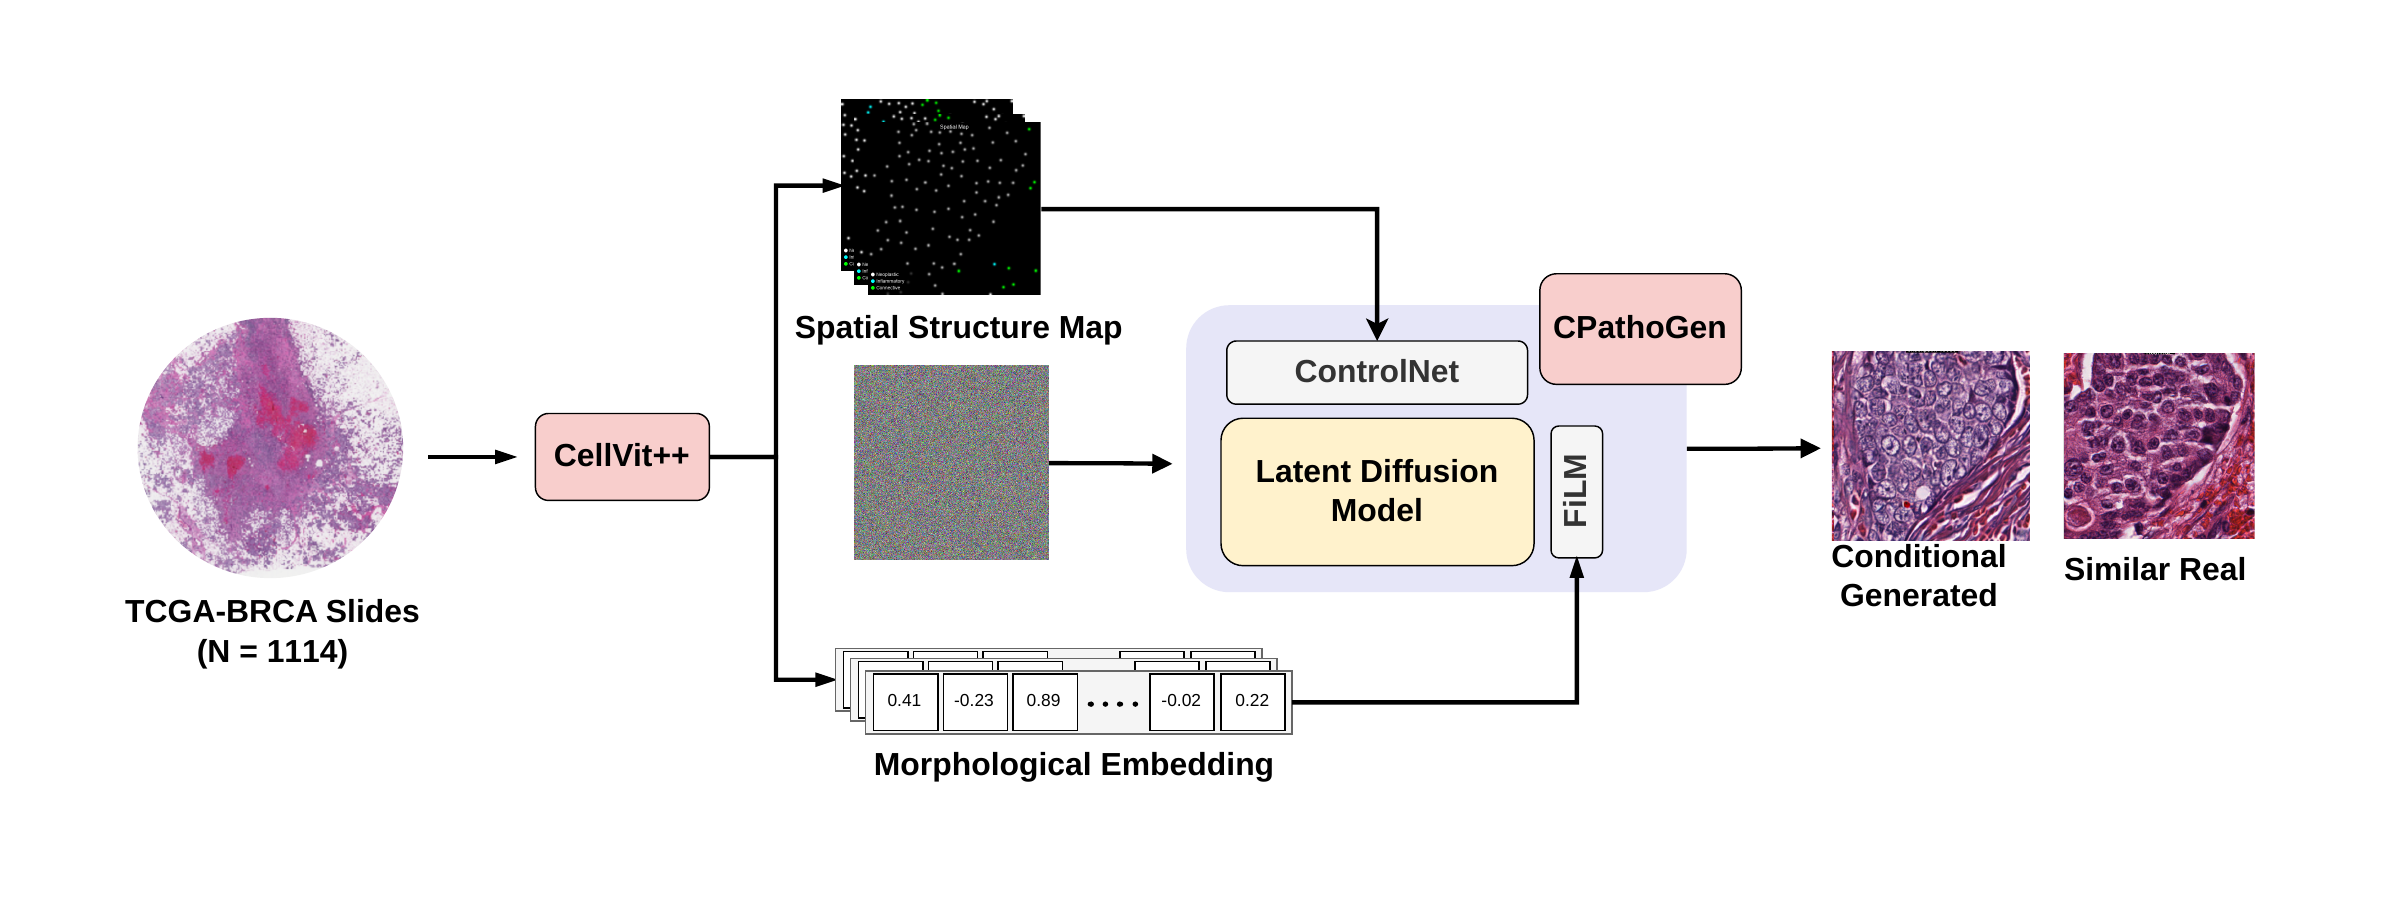
\includegraphics[width=\textwidth,height=0.30\textheight,keepaspectratio]{../related_work/cpathogen_overview.png}
    \vspace{-12mm}
    \caption{\method{} synthesis, selection, auditing, and model probing.}
    \label{fig:overview}
\end{figure*}
